\chapter{Product manual}

\section{Project setup}
The purpose of this section is to support maintenance of the xmd software.

\begin{itemize}
\item install Qt 5.4.0
\item install Qt Installer Framework 1.5.0
\item install Google test
\item install Git
\item install Latex tool
\item clone xMAS repository
\end{itemize}

Once the project is setup, open $''.../xmas/src/main.pro''$ with Qt Creator.
Set xmdmain as default and build the Qt project.

\section{Installer}
The purpose of this section is to support xmd end users who want to design and verify xMAS models.

Go to the xMAS webpage and download the appropriate installer. For example,
choose $''xmd-win-x86-1.0.0.exe''$ for a 32bit MS Windows platform. After
the download was successful, run the installable and follow the procedure.
If the installation is finished, xmd can be started via the desktop icon or the startmenu.

\begin{tcolorbox}[colback=white]
\textbf{
At the moment there is only a Windows installer available and can be found in
the ``installers'' map of the xmas repository.
}
\end{tcolorbox}

\section{xMAS model design}
This section starts with explaining the main parts of the user interface.
Followed by an explanation of the settings and finally how to create and save an
xMAS model.

\subsection{Main window}
Figure~\ref{fig:mainwindow} is the main window of the designer application. On
top there is the xMAS toolbar while in the center it has a single page canvas
that can be setup. A tabbed console can be found at the bottom, the first tab
selects the designer console. Every verification tool loaded as plug-in will get a
console with control panel that can be selected via a tab named as the plug-in.

\begin{figure}[here]
\begin{center}	
	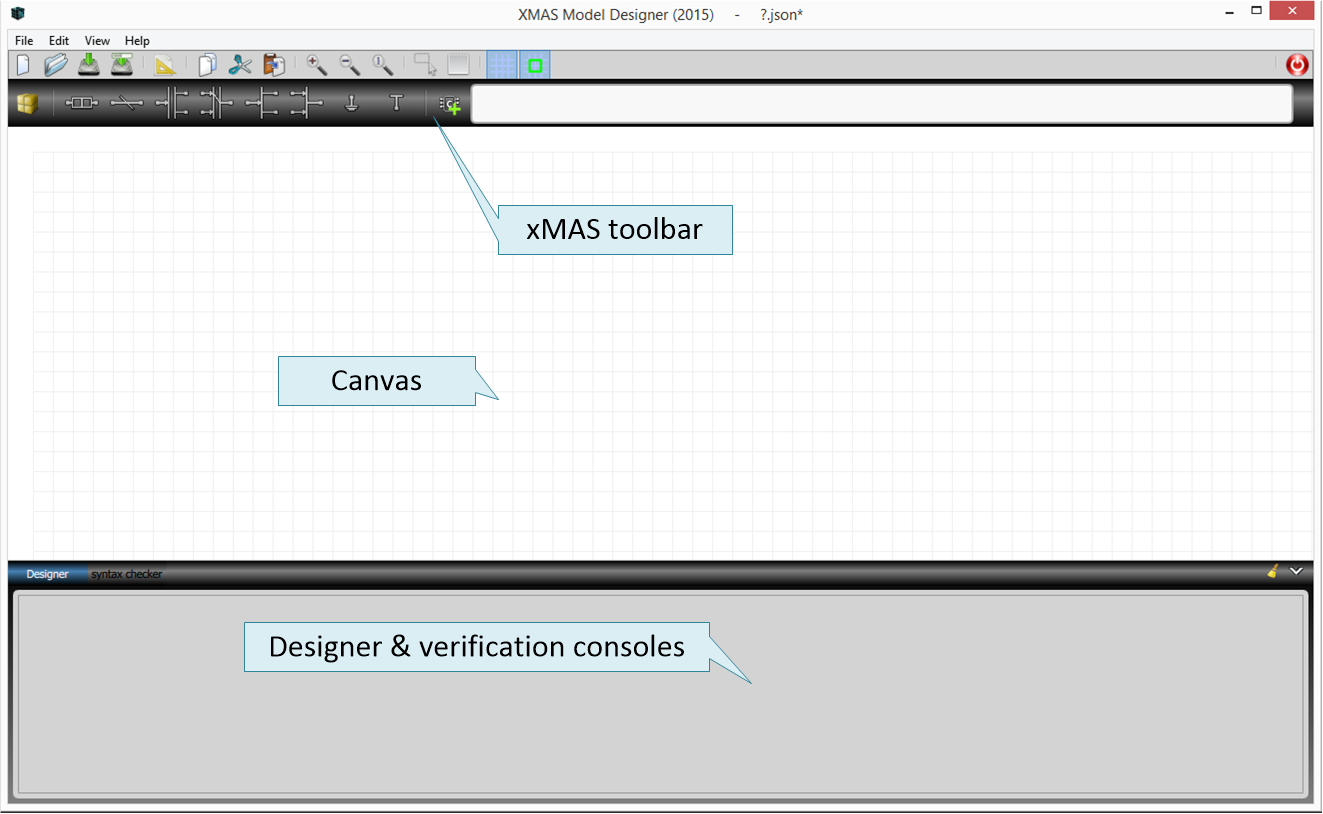
\includegraphics[width=.70\linewidth]{pictures/xmd-empty}
	\caption{Main application window}
	\label{fig:mainwindow}
\end{center}
\end{figure}

\subsection{xMAS tool bar}
The xMAS toolbar (figure~\ref{fig:xmas-toolbar}) holds the items that can be
used to create a model. The packet setup button opens a dialog to set up the
model packet. The xMAS language has only eight primitive components and can be
found next to the packet button. 

\begin{figure}[here]
\begin{center}	
	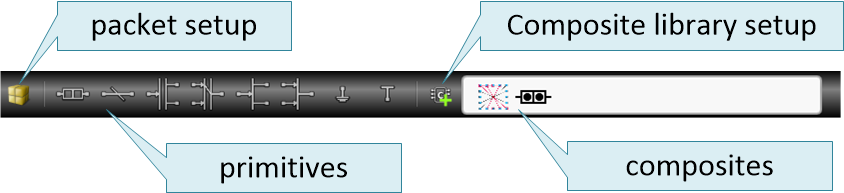
\includegraphics[width=.70\linewidth]{pictures/xmas-toolbar}
	\caption{xMAS toolbar}
	\label{fig:xmas-toolbar}
\end{center}
\end{figure}

Composite components can be found at the right part of this toolbar. Primitive
and composite components can be placed on the canvas by dragging. The area
holding the available composites is called the library which is a horizontal
flickable list. The button at the left side of this list opens a dialog to add a
composite to the library. To remove a composite simply right click the composite
and select remove. Notice that a composite can only be removed if it is not
used.


\subsection{Canvas}
The canvas is a flickable single page, the actual view port can be changed by
drag or swipe it. The size of the canvas page can be changed in the model setup
dialog and is saved with the model. The minimum size is 500 by 500 while the
maximum size is 5000 by 5000. This means that the largest models can directly
hold 500 normal scaled primitive components or 2000 if small scaled.

\paragraph{With grid and snap}canvas items can be easily aligned. The main
toolbar has two toggle buttons, one to show or hide the canvas grid and one to
set the grid snap ``on'' or ``off''. 

\begin{figure}[here]
\begin{center}	
	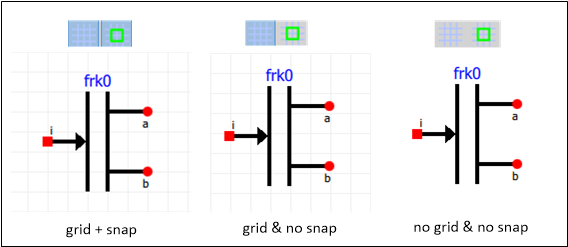
\includegraphics[width=.70\linewidth]{pictures/canvas-grid}
	\caption{canvas grid \& snap options}
	\label{fig:canvas-grid}
\end{center}
\end{figure}

By setting grid snap off a designer can place or move canvas items freely. If
setting this option to ``on'', then at least one component port will snap to the
grid and cannot be placed somewhere in between.

\paragraph{Selecting}canvas items can be done one by one or via a group select.
A selection can be deleted or moved within the canvas its bounds. To select a
group of canvas items you must enable the `group select'' button in the main
toolbar. This because the canvas page its drag-default is used for scrolling.
If group select is enabled then the canvas drag or swipe is disabled.

\begin{figure}[here]
\begin{center}	
	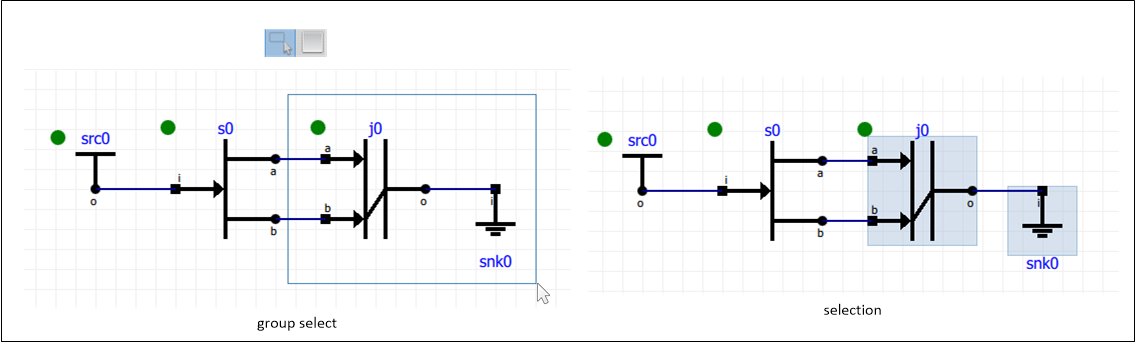
\includegraphics[width=.70\linewidth]{pictures/canvas-selection}
	\caption{canvas group select}
	\label{fig:canvas-selection}
\end{center}
\end{figure}

Next to the ``group select'' button there's a ``select all'' button which selects all
canvas items. Of course all of these actions can be used with standard
shortcuts. Pressing the escape key or click outside the selection will deselect the group.

\paragraph{All components}have common and specific properties. A component
has a name and must be unique. When a component is dragged to the canvas it will
automatically get a unique name. The name can be changed by clicking on it and
press enter when ready. If the name is invalid the change will be ignored. Other
common properties are component size and orientation. Size can be changed in
five steps from 25\% to 400\%. Orientation can be up, down, left and right. Size
and orientation can be set via the context menu or press the left mouse button
and scroll the mouse wheel while hold the ``Ctrl'' or ``Alt'' key. Of course the
touch pad can be used too.

\begin{figure}[here]
\begin{center}	
	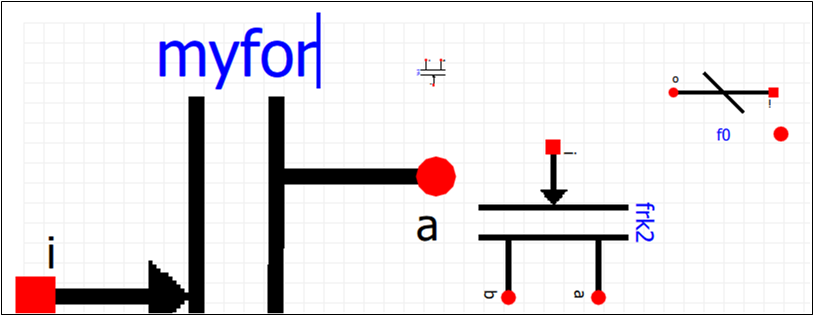
\includegraphics[width=.70\linewidth]{pictures/component-common-properties}
	\caption{canvas common component properties}
	\label{fig:component-common-properties}
\end{center}
\end{figure}

In figure~\ref{fig:component-common-properties}: In-place name editing in
action, small and large size components plus several orientations options are
illustrated. It is also possible to hide or show the component or port names.
These options can be found in the main toolbar or via the canvas context menu.

In figure~\ref{fig:primitives} the graphical representation of the eight
primitive components. Some have a red dot meaning that this component has an
expression to set up. If the expression is valid the dot becomes
green. To open the expression dialog double click on the dot or select it in the
context menu. More information of the expression dialog can be found in the
dialog section~\ref{sec:expression-dialogs}.

\begin{itemize}
\item Queue: In-place size property, a user can only enter digits.
\item Function: Needs a function expression.
\item Fork: No specific properties
\item Join: Need a token expression. Enter 0 or 1 selects the appropriate
input as a restrictive join, otherwise it becomes an unrestrictive join.
\item Switch: Needs a switching expression.
\item Merge: No specific property
\item Sink: Default set as required. A required sink has to be defined later, e.g. outside the composite network.
\item Source: Same as sink but also needs a source expression.
\item Composite: Can be setup with a parametric expression.
\end{itemize}

\begin{figure}[here]
\begin{center}	
	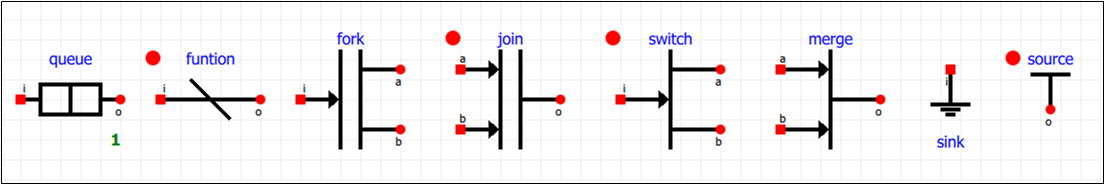
\includegraphics[width=.70\linewidth]{pictures/primitives}
	\caption{list of primitive components}
	\label{fig:primitives}
\end{center}
\end{figure}

\paragraph{A composite} \label{sec:composite} its graphical representation
depends on its model settings, required sinks and sources. If a model is used as
a composite component then all required sinks become outputs and all required
sources become inputs. In other words if a composite network has four required
sinks and three required sources the composite component will have three input
ports at the left and four output ports at the right. In the model setup a user
can also define composite properties. This sets the model its appearance on the
canvas if used as a composite component:
\begin{itemize}
\item The alias is a model nickname and printed in the composite body box.
\item Image is used as a symbol for the composite its body. 
\item If boxed is checked the composite body outline is visible.
Uncheck boxed to let a composite appear as a primitive.
\end{itemize}

\begin{figure}[here]
\begin{center}	
	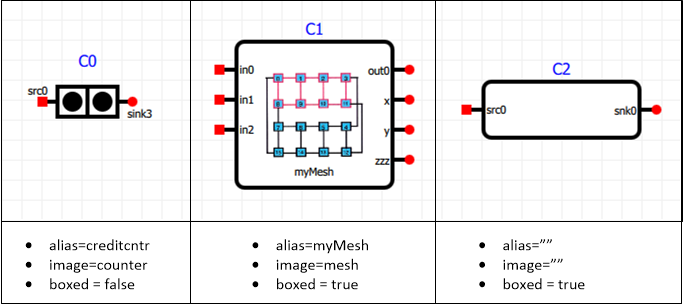
\includegraphics[width=.70\linewidth]{pictures/composites}
	\caption{Composite properties}
	\label{fig:composites}
\end{center}
\end{figure}

The composite at the left in figure~\ref{fig:composites} is un-boxed. For the un-boxed
version the alias will not be printed on the canvas.\\

\begin{tcolorbox}[colback=white]
\textbf{
The symbol for an un-boxed composite must match the default port alignment.
The width is 100 while port spacing is 30.
}
\end{tcolorbox}
\vspace{0.1cm}
The alias is also used as a toolbar tool tip otherwise the filename of the
model-behind is used. A composite that has no symbol gets a default symbol. The
composite at the right in figure~\ref{fig:composites} shows the appearance if no
composite properties were set. A user can always open the composite network and
change its properties. The composite will appear with its new properties in new
and even in existing models.

The port names of a composite are the names of its required sinks and sources.
\begin{tcolorbox}[colback=white]
\textbf{
Try to avoid too long sink and source names so these will fit into the composite its body.
}
\end{tcolorbox}




\subsection{Dialogs}
This subsection gives an overview of all the application specific dialogs. Other
dialogs, e.g. to open or save a model, are native and do not need any further
explanation.
Most dialogs accept with the enter key and cancel with the escape key.

\paragraph{With the application setup dialog} in figure~\ref{fig:app-setup} a
user can change the default model folder. The default model folder is
``xmas-models'' in the users ``home'' directory. A user can select if the
application ask a quit confirm or not. The auto save option will automatically
save the actual modified model every 5 minutes. All these settings are
persistent.\\

\begin{tcolorbox}[colback=white]
\textbf{
It is important to know that models used as composites must be in the same
directory as the main model.
}
\end{tcolorbox}
   
\begin{figure}[t]
\begin{center}	
	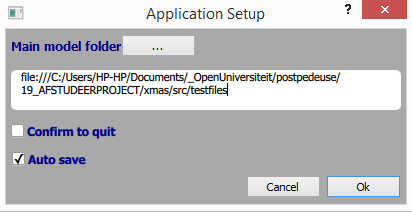
\includegraphics[width=.70\linewidth]{pictures/app-setup}
	\caption{Application setup dialog}
	\label{fig:app-setup}
\end{center}
\end{figure}

\paragraph{The model setup dialog}is used to set the canvas size and the model
filename. Models are saved in json format and therefor the filename must end
with ``.json''. The inputs are checked if valid or not and if not a red border
appears on the entry field. Normally a user does not have to change the folder
because this is set to the application default model folder. But it can become
handy if the user has a sub folder for this modeling project. Composite
properties are optional but useful if this model is meant to be used as a
composite later. Details can be found in the composite paragraph in
section~\ref{sec:composite}. Model size and composite properties are saved in
$''[folder]/[filename]''$. The model setup is shown in
figure~\ref{fig:model-setup}.


\begin{figure}[here]
\begin{center}	
	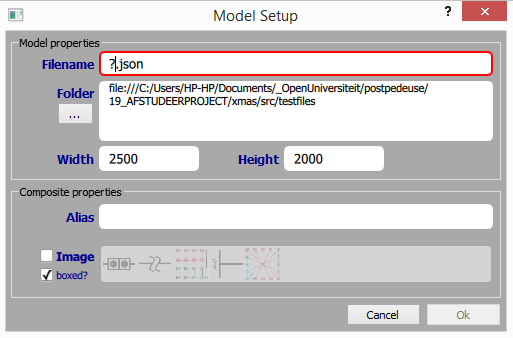
\includegraphics[width=.70\linewidth]{pictures/model-setup}
	\caption{Model setup dialog}
	\label{fig:model-setup}
\end{center}
\end{figure}

\paragraph{The packet setup dialog} is a simple text field entry. It is used to
enter a packet field-range list. The packet is also saved in the model file.
Every field-range entry must start on a new line while field and range are separated with ``\textless ``.
The packet dialog is shown in figure~\ref{fig:packet-setup}.
   
\begin{figure}[here]
\begin{center}	
	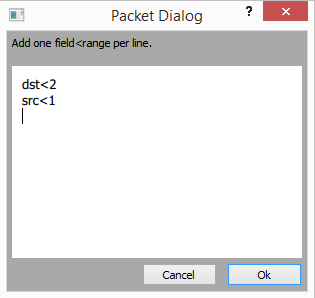
\includegraphics[width=.30\linewidth]{pictures/packet-setup}
	\caption{Packet setup dialog}
	\label{fig:packet-setup}
\end{center}
\end{figure}


\paragraph{Expression dialogs} \label{sec:expression-dialogs}
are used for components that must be set up with
an expression. An expression has a small help on top explaining the syntax and
can differ for each component type. Each time an expression is checked by the
parser and if valid the background becomes green. If the expression is invalid
the background becomes red. The parser will also select the first invalid
character in the expression. A dialog having an invalid expression cannot be
closed with ``ok'' and so not accepted. The expression dialog is shown
in figure~\ref{fig:expression-dialog}.

\begin{figure}[here]
\begin{center}	
	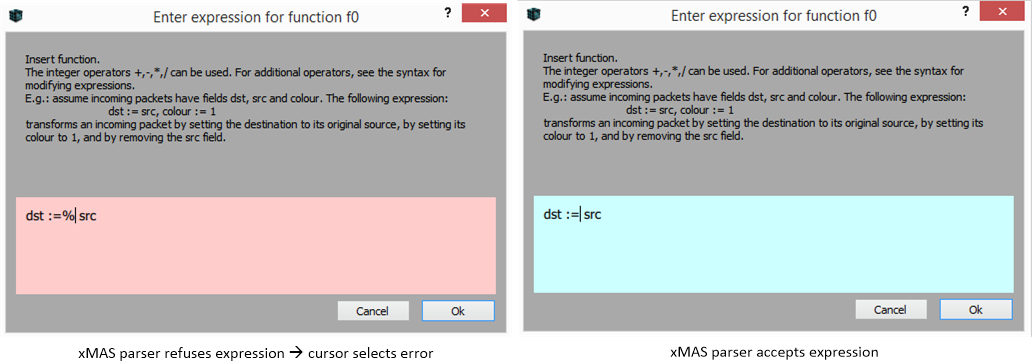
\includegraphics[width=.90\linewidth]{pictures/expression-dialog}
	\caption{Expression dialog}
	\label{fig:expression-dialog}
\end{center}
\end{figure}



\subsection{Designer console}
The designer console is used to print model feedback. The console can be
collapsed, sized or cleared. In figure~\ref{fig:designer-console} you can see an
example of how the expression parser has printed two error messages.

\begin{figure}[here]
\begin{center}	
	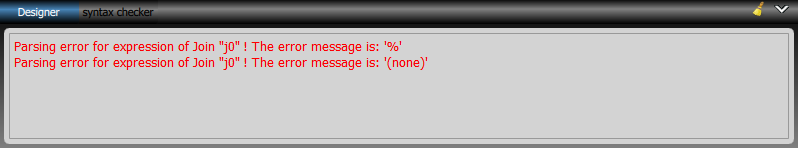
\includegraphics[width=.70\linewidth]{pictures/designer-console}
	\caption{Designer console}
	\label{fig:designer-console}
\end{center}
\end{figure}


\section{xMAS model verification}

The new xMAS designer has a plug-in interface to integrate verification tools.
If a verification tool is build as plug-in then it can be loaded and used from
the xMAS designer. The plug-in interface has a generic structure that can be
implemented into each verification tool. The interface provides:
\begin{itemize}
\item a start signal
\item a stop signal
\item a progress value
\item plug-in specific parameters
\item model reference
\item structured or non-structured text messages
\end{itemize}

Structured messages will not be print on the plug-in console but can be parsed as
in-model-feedback.

To support developers of how to implement the interface into their verification
tools the syntax-checker plug-in can be used as an example. If a verification
tool has the interface, than copy the dll file to the plug-in directory of the
xMAS designer. When the xMAS designer starts it will automatically load all valid
plug-ins from the plug-in directory. Each plug-in will get a console tab.
Figure~\ref{fig:plug-in-console} has one for the syntax checker.

\begin{figure}[here]
\begin{center}	
	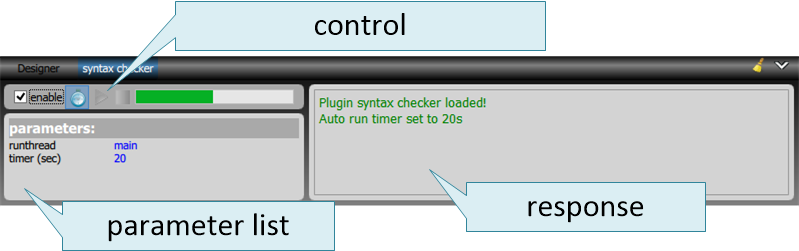
\includegraphics[width=.70\linewidth]{pictures/plug-in-console}
	\caption{Plug-in console}
	\label{fig:plug-in-console}
\end{center}
\end{figure}

\begin{tcolorbox}[colback=white]
\textbf{
In the current project, only the syntax checker has a plug-in interface and can
be used within the designer.
}
\end{tcolorbox}

\paragraph{The plug-in console}has three UI items :
\begin{itemize}
\item The control panel
\item The parameter list
\item The repose list
\end{itemize}

With the control panel a user can send a start or stop to the plug-in. The start
can also triggered by a timer, set by the plug-in interval parameter. For
example in the parameter list of the syntax checker we see that it will run in
the main thread and that it is time triggered every twenty seconds. The control
panel panel also has a progress bar. The parameter list shows all the plug-in
its specific parameters and are read via the interface.

\begin{tcolorbox}[colback=white]
\textbf{
At the moment plug-in parameters cannot be edited via the designer.
}
\end{tcolorbox}


\section{Remarks}
\begin{itemize}
\item The bug list can be found in the appendix or in the Agilefant backlog.
\item The fix list can be found in the appendix or in the Agilefant backlog.
\item Possible features can be found in the appendix or in the Agilefant backlog.
\end{itemize}

